\chapter{Submitted research papers}\label{app:submitted_papers}

A total of three papers have been submitted for peer-review. The peer-review process has not been completed upon final entry of this dissertation. Therefor, they are included in the original state with no peer-review comments implemented.

\section{Experimental Evaluation of Empirical NB-IoT Propagation Modelling in a Deep-Indoor Scenario}
\noindent \textbf{Thrane, J.} \&  Malarski, K. M. \& Christiansen, H. L. \& Ruepp, S. \textit{Experimental Evaluation of Empirical NB-IoT Propagation Modelling in a Deep-Indoor Scenario}. IEEE Globecom 2020, submitted \cite{Thrane2020ExperimentalScenario} 
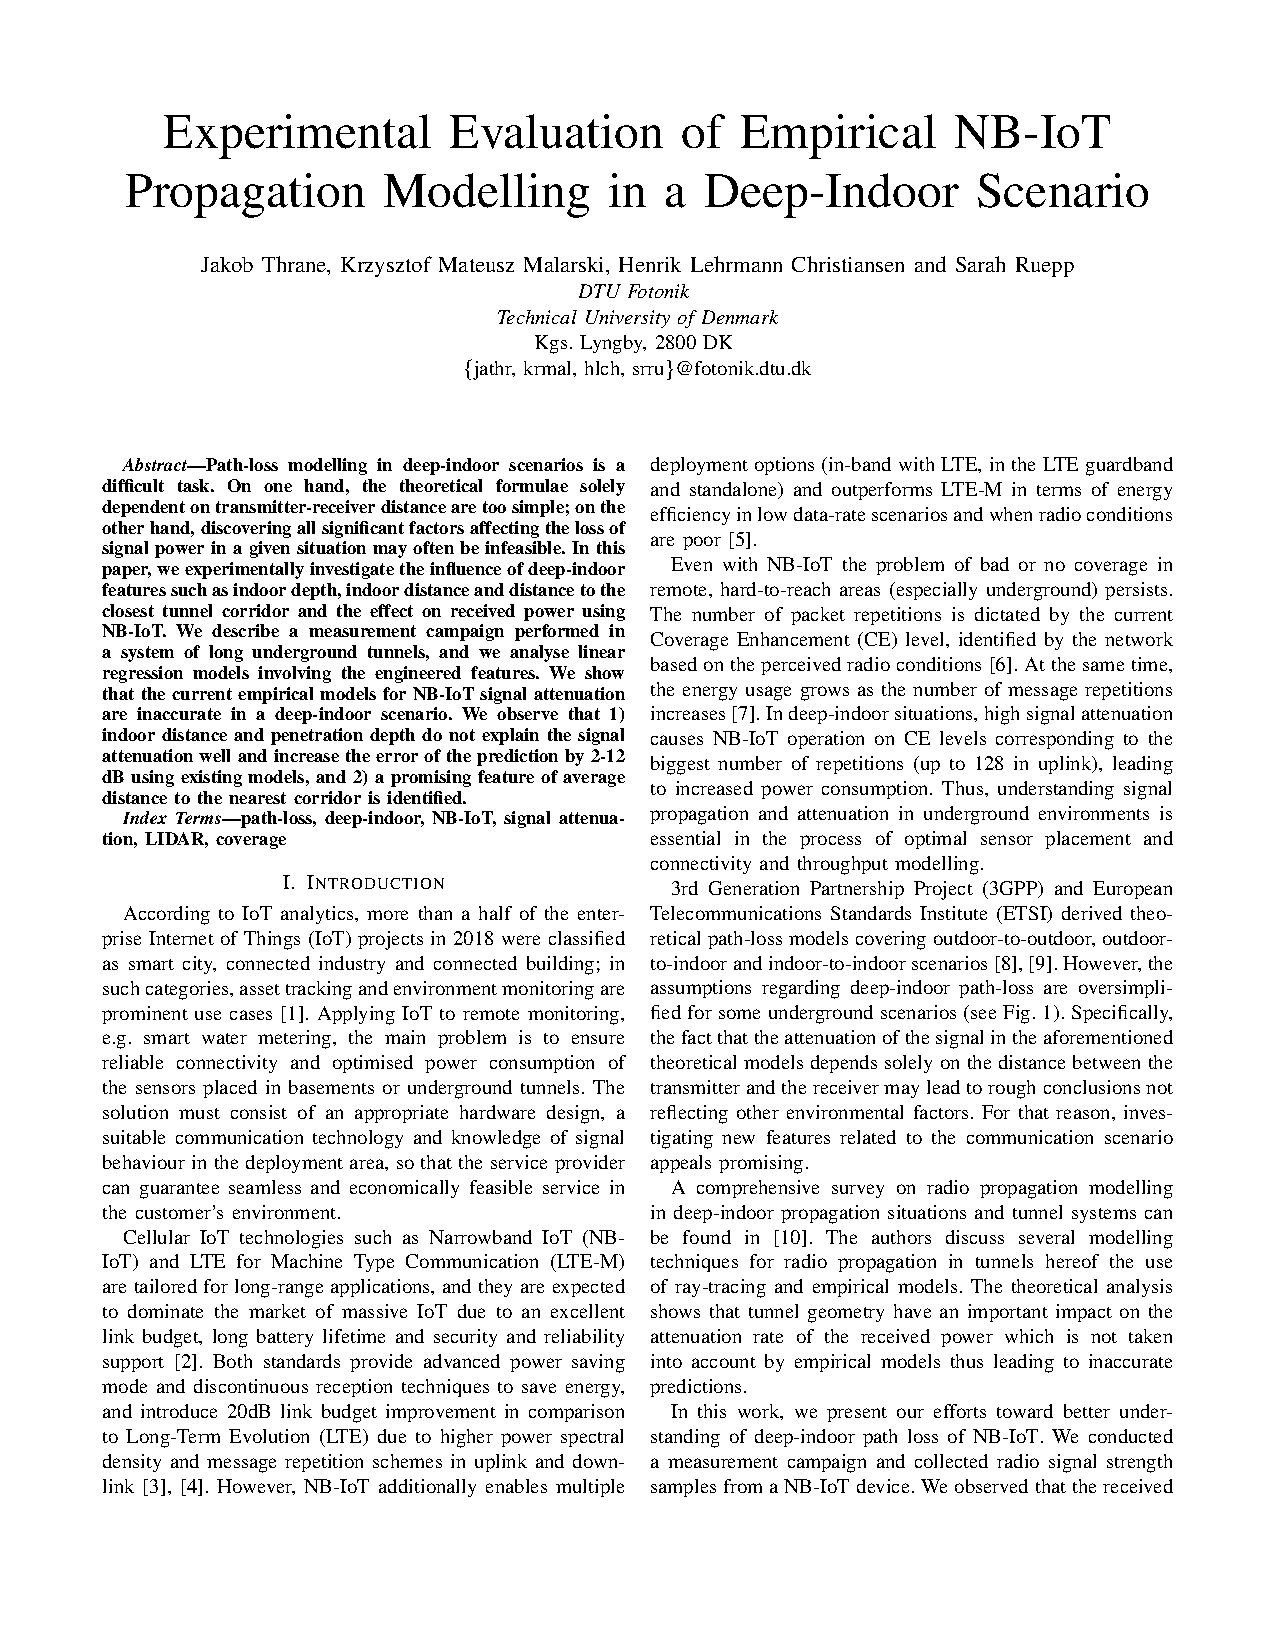
\includepdf[pages=-]{appendix/papers/deep_indoor_paper.pdf}



\section{Pilot Placement Method for Future Cellular Systems in Uplink at 2 GHz using Deep Q-Learning}
\noindent \textbf{Thrane, J.} \& Christiansen, H. L. \textit{Pilot Placement Method for Future Cellular Systems in Uplink at 2 GHz using Deep Q-Learning}. IEEE OJVT 2020, submitted \cite{Thrane2020PilotQ-Learning} 
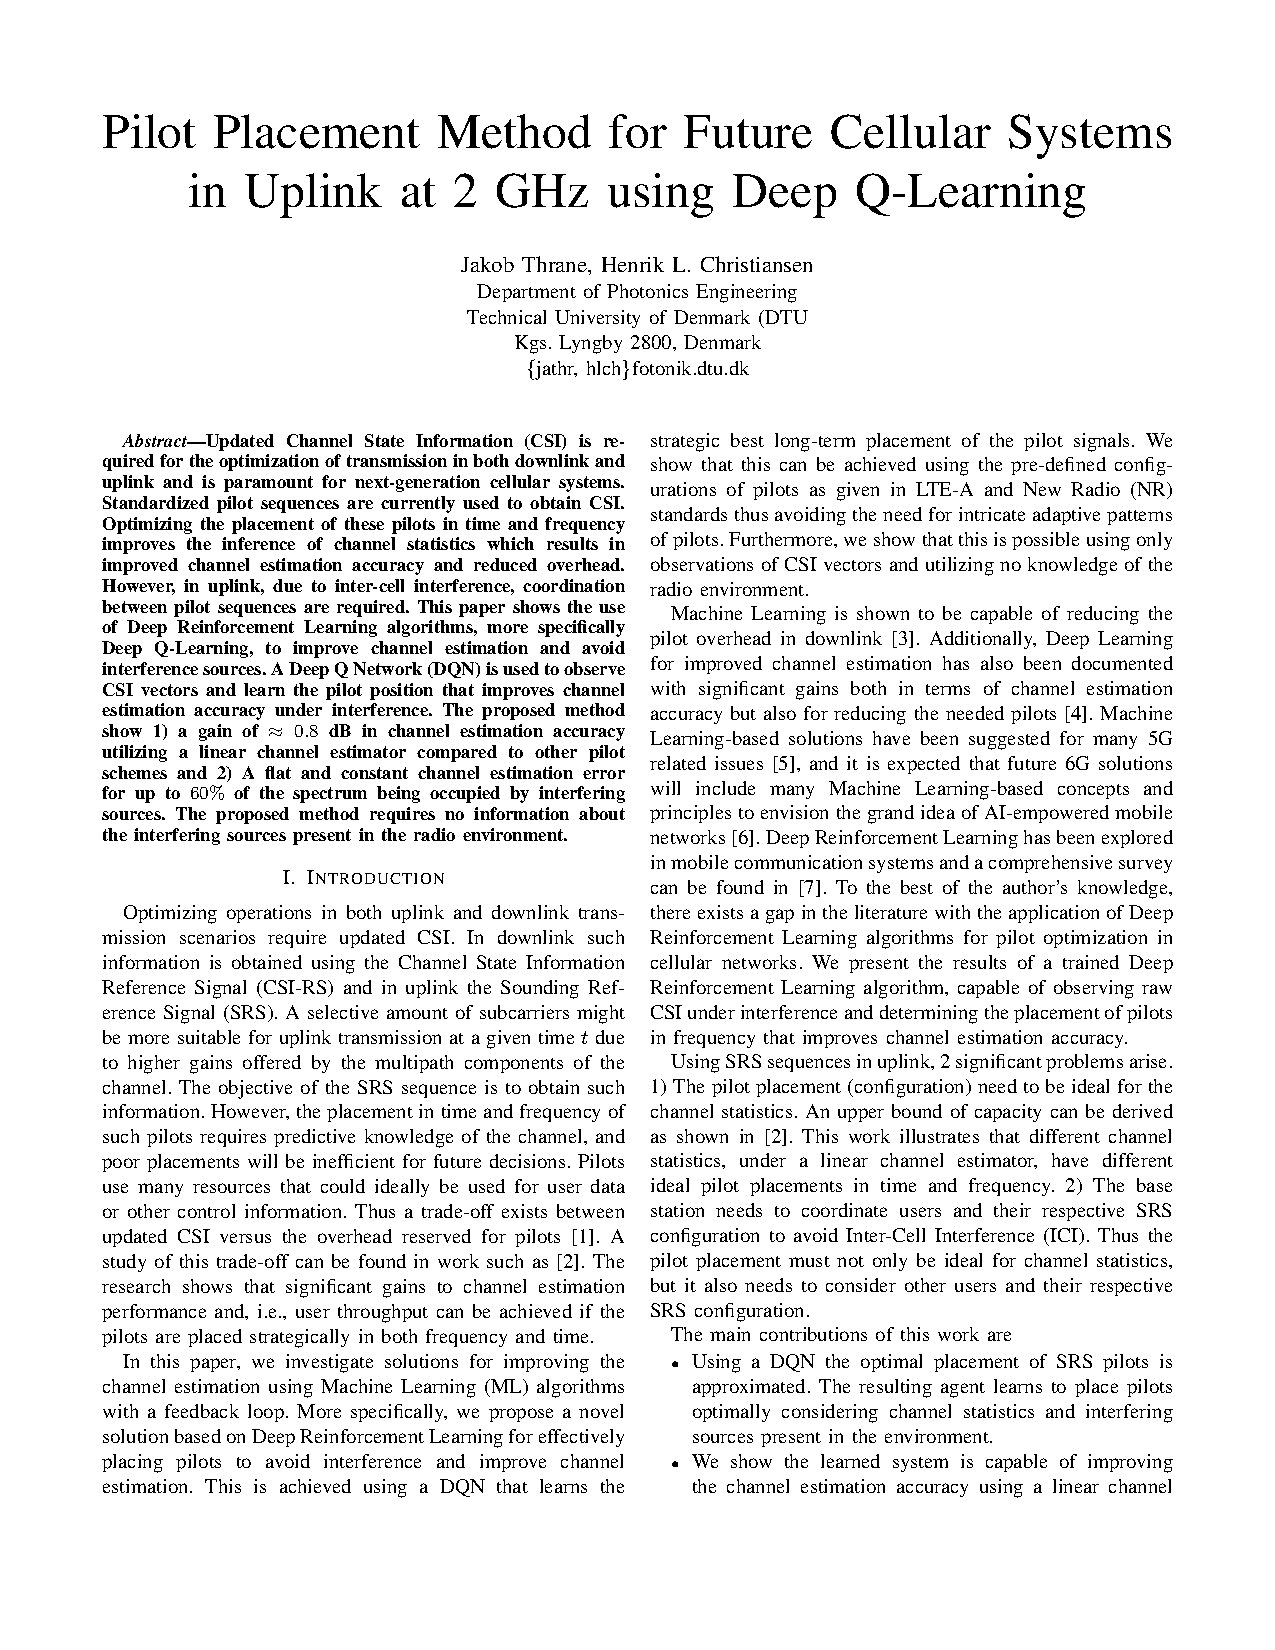
\includepdf[pages=-]{appendix/papers/rl_paper.pdf}




\section{Deep Learning-based Signal Strength Prediction Using Geographical Images and Expert Knowledge}
\noindent \textbf{Thrane, J.} \&  Sliwa, B. \& Wietfeld, C. \& Christiansen, H. L. \textit{Deep Learning-based Signal Strength Prediction Using Geographical Images and Expert Knowledge}. IEEE Globecom 2020, submitted \cite{Thrane2020DeepKnowledge}
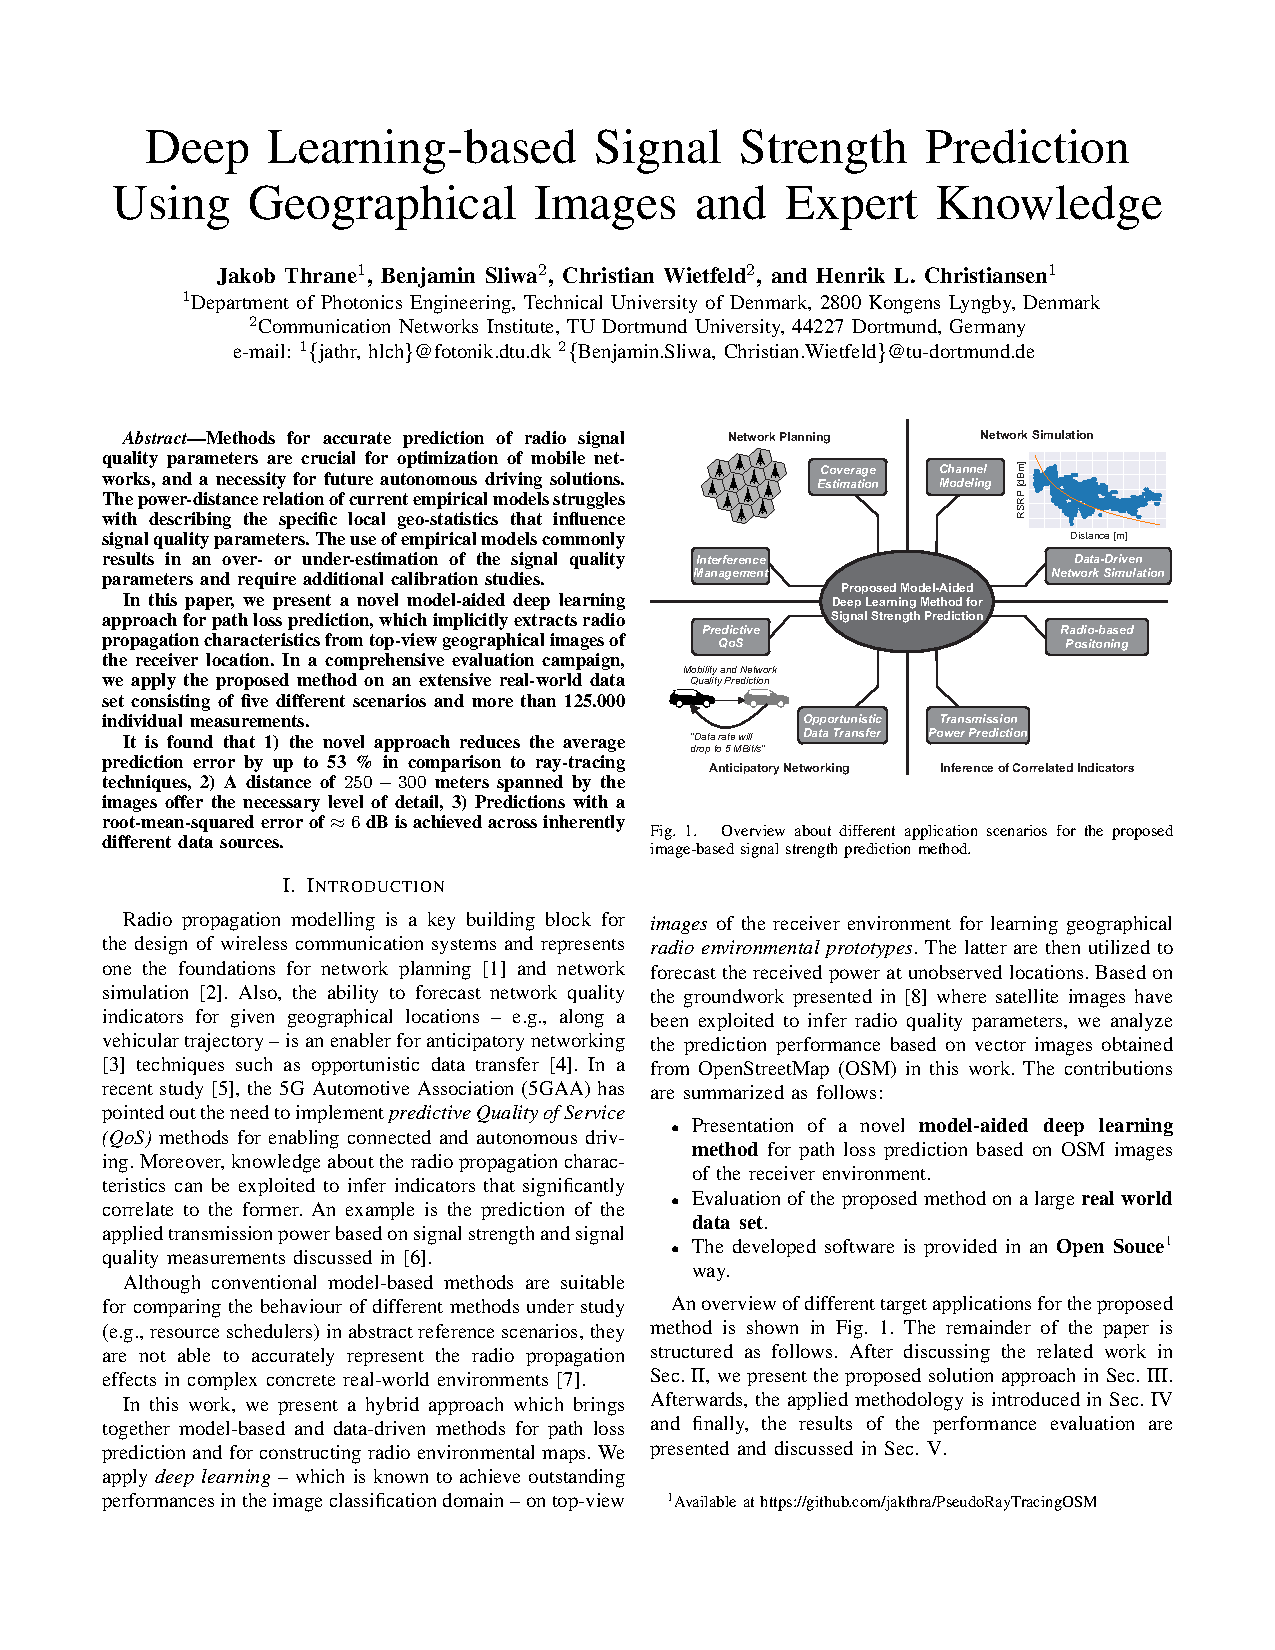
\includepdf[pages=-]{appendix/papers/osm_picture_paper.pdf}